%%%%%%%%%%%%%%%%%%%%%%%%%%%
%	    REFERENCIAS       %
%%%%%%%%%%%%%%%%%%%%%%%%%%%
% http://www.latextemplates.com/
% https://es.wikibooks.org/wiki/Manual_de_LaTeX/Inclusi%C3%B3n_de_gr%C3%A1ficos/Gr%C3%A1ficos_con_TikZ
% https://tex.stackexchange.com/questions/105570/how-to-plot-functions-like-x-fy-using-tikz
\documentclass[10pt]{article}

\usepackage[lmargin=1cm, rmargin=1cm, top=1.5cm, bottom=1.5cm]{geometry}
\usepackage{longtable,multirow,booktabs}
\usepackage{mathrsfs} % para formato de letra
\usepackage[spanish,es-tabla]{babel}
\usepackage[utf8]{inputenc}
\usepackage{newcent}
\usepackage{amsmath}
\usepackage{amsfonts}
\usepackage{amssymb}
\usepackage{graphicx}
\usepackage{float}
\graphicspath{imagenes}
\usepackage{hyperref}
\usepackage{cancel}

\usepackage{sectsty}
\sectionfont{\centering}
\newcommand{\coloredsection}[2]{\section{\color{#1} #2} }

\usepackage{tikz}
\usepackage{pgfplots}
\pgfplotsset{compat=1.15}
\usetikzlibrary{arrows}
\usetikzlibrary{datavisualization}
\usetikzlibrary{decorations.markings}
\renewcommand{\baselinestretch}{1.1}

%%%%%%%%%%%%%%%%%%%%%%%%%%%
%		  TITULO          %
%%%%%%%%%%%%%%%%%%%%%%%%%%%
\title{\bfseries \huge {\rojo{Tarea 3}}}
\author{Ezequiel Remus}
\date{\today}

%%%%%%%%%%%%%%%%%%%%%%%%%%%
%		  INPUTS          %
%%%%%%%%%%%%%%%%%%%%%%%%%%%
%%%%%%%%%%%%%%%%%%%%%%%%%%%%%%%%%%%%%%%%%%%%%%%%%%%%%%%%%%%%
%			 	  Definciciones de Variables               %
%%%%%%%%%%%%%%%%%%%%%%%%%%%%%%%%%%%%%%%%%%%%%%%%%%%%%%%%%%%%
%%%%%%%%%%%%%%%%%%%%%
%     COLORES       %
%%%%%%%%%%%%%%%%%%%%%
\definecolor{R}{RGB}{176, 11, 11}
\definecolor{B}{RGB}{52, 75, 201}
\definecolor{G}{RGB}{20, 176, 18}
\definecolor{M}{RGB}{133, 71, 33}

%%%%%%%%%%%
%  TEXTO  %
%%%%%%%%%%%
\newtheorem{teo}{Teorema}[subsection]
\newtheorem{cor}{Corolario}[subsection]
\newtheorem{defi}{Definición}[subsection]
\newtheorem{obs}{Observación}[subsection]
\newtheorem{propo}{Proposición}[subsection]
\newtheorem{prop}{Propiedad}[subsection]
\newtheorem{ej}{Ejercicio}[subsection]

%%%%%%%%%%%%%%%%%%
%  MATEMATICAS   %
%%%%%%%%%%%%%%%%%%
% Este comando es para conjuntos numericos. Ej: \conj{R}
\newcommand{\conj}[1]{$\mathbb{#1}$ }
% Vectores
\newcommand{\vecAn}[1]{{$(a_1,a_2,\cdots,a_n )$ #1}}
\newcommand{\vecBn}[1]{{$(b_1,b_2,\cdots,b_n )$ #1}}
\newcommand{\vecdos}[2]{{(#1,#2)}}
\newcommand{\vectres}[3]{{(#1,#2,#3)}}
\newcommand{\dom}[1]{{\mathcal{D}}}
\newcommand{\origen}[1]{{$\mathcal{O}$}}
\newcommand{\modulo}[1]{{\vert{#1}\vert}}
\newcommand{\norma}[1]{{\Vert{#1}\Vert}}
\newcommand{\prodesc}[2]{{\langle #1,#2 \rangle}}
\newcommand{\cuerpo}[1]{\textbf{#1}}

\newcommand{\titulo}[1]{\subsection{\underline{\textbf{\color{B}{#1}}}}}
\newcommand{\ejercicio}[1]{\subsection{\textbf{\color{R}{#1}}}}
\newcommand{\solucion}[1]{\fbox{\textbf{Solución}}#1}
\newcommand{\resultado}[1]{\color{G}{#1}}


%%%%%%%%%%%%%%%%%%%%%%%%%%%%%%%%%%%%%%%%%%%%%%%%%%%%%%%%%%%%%%%%
%					Inicio del documento                       %
%%%%%%%%%%%%%%%%%%%%%%%%%%%%%%%%%%%%%%%%%%%%%%%%%%%%%%%%%%%%%%%%
\begin{document}
\renewcommand{\tablename}{Tabla}
\renewcommand{\abstractname}{Enunciado}
%\pagestyle{myheadings}
%TITULO
%modificar el formato del titulo
\maketitle
%\abstractname{Enunciado}
% Here is the abstract.
\begin{abstract}
\caja{1}{0.9}{
	Una bolita de masa $m$ se mueve por un tubo delgado, carente de rozamiento, el cual describe una semicircunferencia de radio $R$. 
	La bolita se halla sujeta por un extremo a un resorte de constante elástica $k$ y longitud natural $l_0 = \frac{\pi R}{2}$, y por el otro a una soga, deslizando ambos elementos por el interior del tubo, tal como muestra la figura. Del extremo de la soga pende, a través de una polea, otro cuerpo de masa $M$ que actúa como contrapeso. 
	Considere la soga inextensible, y las masas de soga, resorte y poleas despreciables. En el instante inicial la bolita se halla en el punto $A (\varphi = 0)$ con velocidad $v_0$.
	\begin{itemize}
		\item[a)] Plantee las ecuaciones de Newton para cada una de las masas. Halle la ecuación diferencial que rige el movimiento de la bolita.
		\item[b)] Halle gráficamente la o las posiciones de equilibrio de la bolita, determinando si corresponden a posiciones de equilibrio estable o inestable.
		\item[c)] Halle la expresión de la fuerza de vínculo ejercida por el tubo sobre la bolita como función del ángulo $\varphi$.	
	\end{itemize}
	}
\end{abstract}

%---------------------------------------------------
%	ITEM 0
\coloredsection{MetallicGold}{Esquemas, Diagramas, Vinculos}
Voy a empezar haciendo las figuras y analizando los vinculos entre los curpos. 
\begin{figure}[h]
\caja{1.25}{0.35}{
	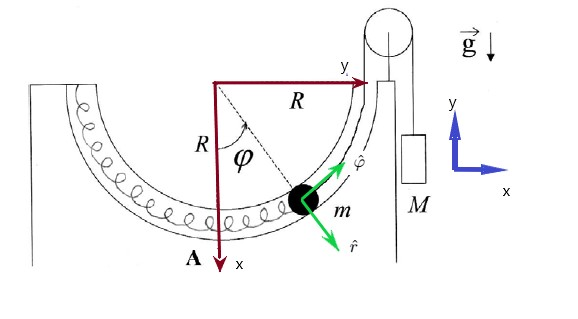
\includegraphics[scale=0.5]{figuras/esquema.jpg}
	\caption{Planteo de coordenadas}
}
\caja{1}{0.3}{
	\centering
	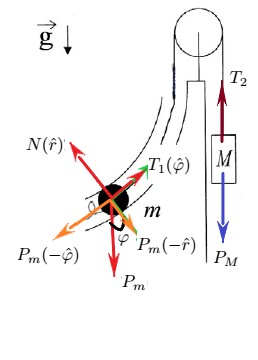
\includegraphics[scale=0.6]{figuras/dcl.jpg}
	\caption{Diagramas de cuerpo libre}
}
\caja{1.22}{0.25}{
	\centering
	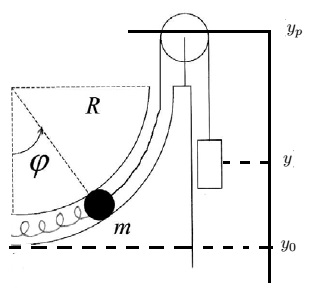
\includegraphics[scale=0.5]{figuras/soga.jpg}
	\caption{Parametros para el calculo de la soga}
}
\end{figure}
Ahora, con respecto a los vinculos. Tenemos una soga inextencible y sin masa. Al ser inextensible, lo que nos dice es que su songitul $L_s$ es constante. 
Por otro lado, su longitud $L_s$ viene dada por:
\[L_s = \overbrace{(\frac{\pi R}{2} - R \varphi) + (y_p - y_0)}^{Parte \hspace{0.1cm} dentro \hspace{0.1cm} del \hspace{0.1cm} bucle} + \underbrace{(y_p - y)}_{Entre\hspace{0.1cm} la \hspace{0.1cm} polea \hspace{0.1cm} y \hspace{0.1cm} M} + \overbrace{(\pi r_p)}^{Sobre \hspace{0.1cm} la \hspace{0.1cm} polea}\]
\[ Con: \hspace{0.3cm}  y_0 = -\frac{\pi R}{2}\]

Donde $(\frac{\pi R}{2} - R \varphi)$, corresponde a la posición de la bola de masa $m$ resoecto de como mediriamos la soga. y $y_0$ corresponde a un punto inicial de como medimos a la soga dentro del medio arco si la bola se encontrase en el punto $A$ de la \textit{figura 1}.

Con esto se obtiene:  
\[L_s = - R \varphi + y_p  + (y_p - y) + \pi r_p\]
Como dijimos, la soga es inextensible, por lo que $\dot{L}_s = 0 $ y $\ddot{L}_s = 0$. Como $y_p$ que corresponde a la posición de la polea, es un punto fijo sus derivadas son $\dot{y}_0= 0$, $\ddot{y}_0= 0$, no asi con la variable $y$ la cual nos indica como se mueve la masa $M$. 

Además, $\pi r_p$ es una cantidad constante,la cual representa al pedaso de soga que estara sobre la polea ($r_p$ = radio de la polea), por lo que al derivar se nos anula y por ultimo con $- R \varphi$, tenemos que $R$ es constante pero $\varphi$ no, pues este cambia a medida que cambia $y$ por el vinculo entre la soga y la bola de masa $m$. Por lo tanto, si derivamos $L_s$ dos veces, nos queda que:  
\[\ddot{L_s} = - R \ddot{\varphi}  - \ddot{y} = 0 \hspace{0.2cm} \sii \hspace{0.2cm} \rojo{\ddot{y} = - R \ddot{\varphi}} \hspace{0.3cm} (1)\]
La ecuación (1) nos da un vinculo entre las aceleraciones de los con masa $m$ y $M$ a partir de aproximar que la soga no se estira, ni contrae.

Por otro lado, el hecho de que la soga no tenga masa, y teniendo en cuenta la disposición de sus extremos nos grantiza la relación:
\[m_s a_t \underbrace{=}_{m_s = 0} 0 = T_1 - T_2 \hspace{0.2cm} \sii \hspace{0.2cm} \rojo{T_1 = T_2}\hspace{0.3cm} (2) \]
Con esto obtenemos un vinculo que nos relaciona a ambas tensiones y que nos garantiza que sus modulos son iguales.

%---------------------------------------------------
%	ITEM A
\coloredsection{MetallicGold}{Item a}

Teniendo en cuenta los diagramas de cuerpo libre, las coordenadas tomadas y los vinculos establecidos en la sección anterior, podemos encontrar las ecuaciones de Newton para ambos cuerpos.

Empecemos por la Bola atada al resorte. Esta bola, esta engarzada a un resorte y enganchada de alguna forma a una soga. Además esta apoyada sobre una superficie circular la cual nos permite describir el movimiento de la bolita en coordenadas polares. Luego, como hay gravedad y la bolita tiene masa obviamente actua el peso y en reacción a estar apollada a la superficie circular tendremos la normal a la superficie. Al descomponer todas estas fuerzas en coordenadas polares como se indica en la \textit{figura 2}, se puede verificar que las ecuaciónes de Newton vienen dadas por:
\[Bola: \left\lbrace \begin{array}{lll}
\hat{r}: & N - m g \cos{(\varphi)} = -m R \dot{\varphi}^2 & (3)\\
\hat{\varphi}: & T_1 - m g \sin{(\varphi)} - kR \varphi = m R \ddot{\varphi}&(4)
\end{array}\right.\]
Notemos que para el estiramiento del resorte tuvimos en cuenta solo su desplazamiento desde el punto $A$ hasta el punto $R \varphi$, esto es así tomando como punto de partida
dicho punto. Si ubiesemos, por ejemplo tomado al eje $x$ en el extremo superior de la semicircunferencia tendriamos que sumarle su longitud natural $l_0 = \frac{R\pi}{2}$.

Vamos ahora con la masa $M$. Esta tiene simplemente un movimiento vertical el cual se da justamente porque la soga esta totalmente tensa, si esto no fuese asi, quizas tendria un bamboleo hacia los costados como si fuese un movimiento del estilo del pendulo, pero por suelte no es el caso. 

En particular, vemos que solo actuan la tension de la soga en orientación positiva sobre el eje $y$ y en orientación negativa para el peso. Tenemos asi que:
\[\hat{y}: \hspace{0.2cm} T_2 - M g = M \ddot{y} \hspace{0.5cm} (5)\]

Luego, utilizando los resultados obtenidos por los vinculos y las ecuaciones $(4)$ y $(5)$ podemos obtener la ecuación de movimiento de este sistema.

Primero, notando por (2) que las tensiones son iguales, podemos despejar $T_2$ de la ecuación (5). Además, tenemos la ecuación (1) que nos establece el vinculo entre las aceleraciones de ambos cuerpos. Por lo tanto, con esto podemos deducir lo siguiente:
\[T_2 - M g = M \ddot{y} \underbrace{=}_{Aplico (1)} T_2 - M g = - M R \ddot{\varphi} \hspace{0.2cm} \sii \hspace{0.2cm} \rojo{T_2  =  M g - M R \ddot{\varphi}} \hspace{0.2cm} (6)  \] 
Tenemos una ecuación para la tensión y como por vinculos habiamos llegado a que $T_1 = T_2 = T$, podemos reemplazar la ecuación (6) en la ecuación (4) y así obtener una ecuación para el movimiento del sistema.

\[T_1 - m g \sin{(\varphi)} - kR \varphi = m R \ddot{\varphi} \hspace{0.2cm} \underbrace{\sii}_{T_1 = T_2} \hspace{0.2cm} M g - M R \ddot{\varphi} - m g \sin{(\varphi)} - kR \varphi = m R \ddot{\varphi}\]
Despejando y agrupando, obtenemos la siguiente ecuación:
\[(M-m \sin{(\varphi)}) g - K R \varphi = (m+M) R \ddot{\varphi} \hspace{0.2cm} \sii \hspace{0.2cm} 
\rojo{\frac{(M-m \sin{(\varphi)}) g}{(m+M) R} - \frac{K}{(m+M)} \varphi = \ddot{\varphi}} \hspace{0.2cm} (7)\]
Luego, la ecuación (7) es la ecuación diferencial que rige el movimiento.
%---------------------------------------------------
%	ITEM B
\coloredsection{MetallicGold}{Item b}
La posición de equilibrio de un sistema, viene dada cuando la aceleración del sistema en dicha posición es cero. 

Podemos calcular las posibles posiciones de equilibrio a partir de la ecuación (7) buscando analiticamente que valores de $\varphi$ cumplen con la ecuación para $\ddot{\varphi} = 0$.

Entonces, de (7):
\[\frac{(M-m \sin{(\varphi_{eq})}) g}{(m+M) R} - \frac{K}{(m+M)} \varphi_{eq} = 0 \hspace{0.2cm} \sii \hspace{0.2cm} \frac{(M-m \sin{(\varphi_{eq})}) g}{\cancel{(m+M)} R} = \frac{K}{\cancel{(m+M)}}\varphi_{eq} \hspace{0.2cm} \sii \hspace{0.2cm} \]
\[\sii \hspace{0.2cm} (M-m \sin{(\varphi_{eq})}) g  = K R \varphi_{eq} \hspace{0.2cm} \sii \hspace{0.2cm} Mg - mg \sin{(\varphi_{eq})} = K R \varphi_{eq}  \hspace{0.2cm} \sii\]
\[\sii \hspace{0.2cm} \rojo{\sin{(\varphi_{eq})} = -\frac{K R}{m g} \varphi_{eq} + \frac{M}{m}} \hspace{0.2cm} (8)\]
Vemos en la ecuación (8) que, si se cumple esa igualdad para ciertos valores de $\varphi_{eq}$, entonces el equilibrio sera posible en esas posiciónes. 

Vemos que de un lado de la igualdad tenemos a la función seno y del otro lado una recta de pendiente negativa cuya ordenada al origen es una relación entre las masas.

Si graficamos esto, podemos ver algo similar a esto :

Por como tenemos definido el sistema de coordenadas, podemos interpretar que la bola, si pudiese recorrer toda la semicircunferencia, recorreria los $\varphi$ dentro del intervalo $[\frac{-\pi}{2}, \frac{\pi}{2}]$.

\begin{figure}[h]
	\centering
	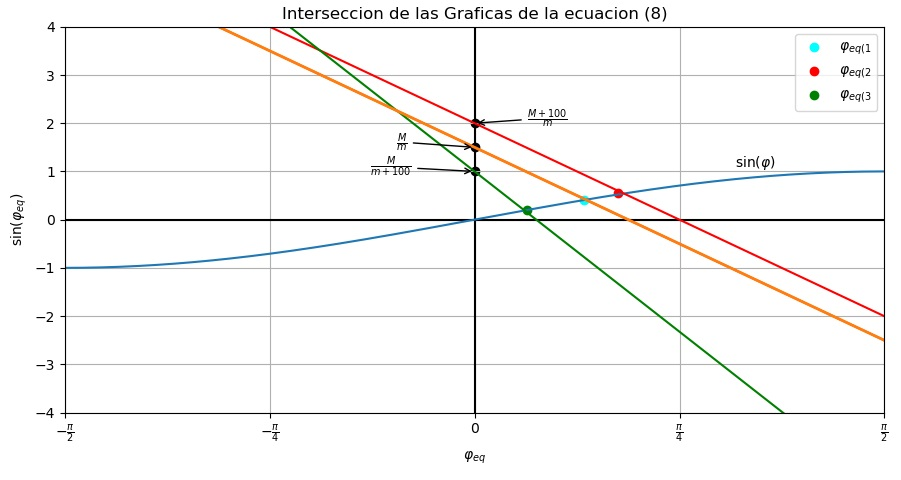
\includegraphics[scale=0.7]{figuras/graf1.jpg}
	\caption{Variación de masas $M$ y $m$ y variación del grafico}
\end{figure}
En esta primer imagen, podemos ver como varia la recta al variar sobre una constante (la cual en el grafico esta representada por el valor de 100) los valores de ambas masas\footnote{En las referencias hay un link a un repositorio donde esta el codigo de los graficos en donde se pueden variar $k$,$R$,$m$ y $M$ para ver que pasa}.  

En la ecuación vemos que al variar $M$ solo afectaremos a la ordenada al origen, mientras que al variar $m$ cambiamos tanto el valor de la ordenada como el valor de la pendiente. Luego, al variar los valores de $k$ o de $R$ tambien camiaremos la pendiente.

Sabemos que, en particular, las posiciones de equilibrio se dan en la intersección de las rectas con la función seno, las cuales en las figuras estan indicados por los puntos, rojo, verde y celeste.

Analisemos analiticamente en que casos sera posible un equilibrio para el sistema. Volvamos a la ecuación (8).

La pendiente al ser negativa siempre, a menos claro que $\varphi$ sea negativo, esto solo pasaria para valores de k muy muy grandes, por lo que nos quedaremos con el intervalo para $\varphi = [0, \frac{\pi}{2}]$, o sea el sistema tendra libertad de movimiento desde el punto $A$ hasta la parte superior del lado derecho de la semicircunferencia. Pasando a cuentas este hecho tenemos:
\[0 \menig \varphi_{eq} \menig \frac{\pi}{2} \hspace{0.2cm} \sii \hspace{0.2cm} 0 \menig \sen{(\varphi_{eq})} \menig 1 \hspace{0.2cm} \sii \hspace{0.2cm}\]
\[\hspace{0.2cm} \sii \hspace{0.2cm} 0 \menig -\frac{K R}{m g} \varphi_{eq} + \frac{M}{m} \menig 1 
  \hspace{0.2cm} \sii \hspace{0.2cm} 0 \menig -\frac{K R + Mg}{m g} \varphi_{eq} \menig 1 
  \hspace{0.2cm} \sii \hspace{0.2cm} 0 \menig -K R \varphi_{eq} + Mg \menig m g 
\]  
\[\hspace{0.2cm} \sii \hspace{0.2cm} - Mg \menig -K R \varphi_{eq} \menig m g - Mg 
\hspace{0.2cm} \sii \hspace{0.2cm} Mg \mayig K R \varphi_{eq} \mayig   Mg - m g  
\]
\[\hspace{0.2cm} \sii \hspace{0.2cm} \rojo{\frac{Mg}{K R} \mayig  \varphi_{eq} \mayig   \frac{Mg - m g}{K R}} \hspace{0.3cm} (9)\]
 En particular, lo que nos dice la ecuación (9) es que para que exista una posición de equilibrio, esta debe estar comprendida dentro de los valores de las variables que cumplen dicha desigualdad.
  
  \textbf{¿Que pasa si $\varphi_{eq} = 0$?:}
  
  Tendriamos la situación siguiente en la ecuación (8).
  \[\sin{(0)} = -\frac{K R}{m g} \cdot 0 + \frac{M}{m} \hspace{0.2cm} \sii \hspace{0.2cm} 0 = 0 + \frac{M}{m}\]
  Notemos que esto se da solamente cuando quitamos la masa $M$, de otra forma seria un absurdo.
  
  \textbf{¿Que pasa si $\varphi_{eq} = \frac{\pi}{2}$?:}
  
  Tendriamos la situación siguiente en la ecuación (8).
  \[\sin{(\frac{\pi}{2})} = -\frac{K R}{m g} \cdot \frac{\pi}{2} + \frac{M}{m} \hspace{0.2cm} \sii \hspace{0.2cm}
  	1 + \frac{K R}{m g} \cdot \frac{\pi}{2} = \frac{M}{m} \hspace{0.2cm} \sii \hspace{0.2cm}
    \frac{K R + mg}{m g} \cdot \frac{\pi}{2} = \frac{M}{m} \hspace{0.2cm} \sii \hspace{0.2cm}
     	(K R + mg) \frac{\pi}{2} = M g 
   \]
   Lo cual, en principio no hay nada que me impida esta posibilidad, solo necesitamos un peso para $M$ lo suficientemente grande como para vencer las fuerzas realizadas por el resorte y la bola.
   
   Entonces, en particular tenemos los siguientes tres casos a anlazisar:
\begin{enumerate}
	\item $\varphi_{eq} = 0$
	\item $\varphi_{eq} : \frac{Mg}{K R} \mayig  \varphi_{eq} \mayig   \frac{Mg - m g}{K R}$
	\item $\varphi_{eq} = \frac{\pi}{2}$
\end{enumerate}     
  
  Ahora, analisemos la estabilidad. Recordemos que para analizar la estabilidad de un equilibrio debemos ver la derivada de la fuerza respecto de la posición y analizar cual sera su signo.
  
  Derivemos la ecuación de movimiento:
  \[\frac{d \ddot{\varphi}}{d \varphi} = -\frac{K}{(m+M)} - \frac{mg}{(m+M)R} \cos{(\varphi)}\]		 
 Recordemos el criterio de estabilidad segun el signo de la derivada:
 \[\frac{d \ddot{\varphi}}{d \varphi} = \left\lbrace \begin{array}{lll}
 > 0 & \implica & inestable \\
 = 0 & \implica & (analiso \hspace{0.2cm} la \hspace{0.2cm} siguiente \hspace{0.2cm} derivada \hspace{0.2cm} y \hspace{0.2cm} sigo \hspace{0.2cm} el \hspace{0.2cm} criterio \hspace{0.2cm} otra \hspace{0.2cm} vez) \\
 < 0 & \implica & estable
 \end{array}\right.\]
  Analisemos la derivada para los diferentes casos:
  \begin{itemize}
  	\item[•] \textbf{$\varphi_{eq} = 0$}:
  	\[\frac{d \ddot{\varphi}}{d \varphi}\left\vert_{\varphi_{eq} = 0}\right. = -\frac{K}{(m+M)} - \frac{mg}{(m+M)R} \cos{(0)} = -\frac{K}{(m+M)} \rojo{< 0}\]
  	$\therefore$, es estable
  	
  	\item[•] \textbf{$\varphi_{eq} = \frac{\pi}{2}$}  	
  	\[\frac{d \ddot{\varphi}}{d \varphi}\left\vert_{\varphi_{eq} = \frac{\pi}{2}}\right. = -\frac{K}{(m+M)} - \frac{mg}{(m+M)R} \cos{(\frac{\pi}{2})} = -\frac{K}{(m+M)} - \frac{mg}{(m+M)R} \rojo{< 0}\]
  	$\therefore$, es estable
  	\item[•] \textbf{$0 < \varphi_{eq} < \frac{\pi}{2}$}
	Ahora, si lo pensamos matematicamente. Como la funcion es continua y en los extremos tiende a ser estable, en los valores intermedios deberia pasar lo mismo.
	
	Planteemos entonces que la derivada es negativa y fijemonos si coincide con lo obtenido en la ecuación (9).
	\[-\frac{K}{(m+M)} - \frac{mg}{(m+M)R} \cos{(\varphi)} < 0 
	\hspace{0.2cm} \sii \hspace{0.2cm} -\frac{K}{\cancel{(m+M)}} < \frac{mg}{\cancel{(m+M)}R} \cos{(\varphi)}
	\hspace{0.2cm} \sii \hspace{0.2cm}
	\]
	\[\hspace{0.2cm} \sii \hspace{0.2cm} -\frac{K R}{mg} <  \cos{(\varphi)} \hspace{0.2cm} \sii \hspace{0.2cm} -\frac{K R}{mg} \frac{1}{\cos{(\varphi)}} < 1 \]
	 Veamos que pasa graficamente con la función coseno para nuestro sistema:
	\begin{figure}[h]
	\centering
	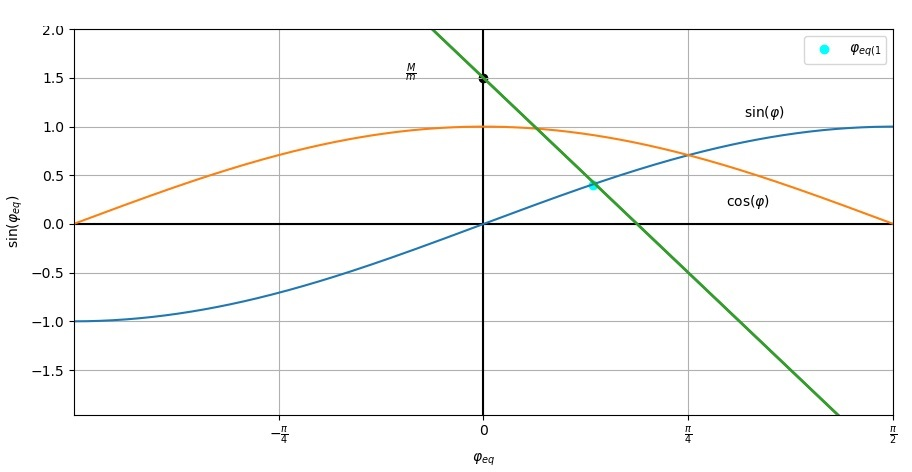
\includegraphics[scale=0.7]{figuras/graf2.jpg}
	\caption{Grafica del seno, coseno y recta establesidas}
\end{figure} 
	Fijemosnos, que si multiplicamos por el seno a ambos lados, nos queda lo siguiente:
	\[-\frac{K R}{mg} \tan{(\varphi_{eq})} < \sen{(\varphi_{eq})}\]
	y en particular, sabemos que el seno es menor que $1$, entonces:
	\[-\frac{K R}{mg} \tan{(\varphi_{eq})} < \sen{(\varphi_{eq})} \menig 1\]
	Ahora, recordando la ecuación (8):
	\[-\frac{K R}{mg} \tan{(\varphi_{eq})} < -\frac{K R}{m g} \varphi_{eq} + \frac{M}{m} \menig 1\]
	En particular esto ya lo habiamos visto mas arriba, cuando calculamos los $\varphi_{eq}$ posibles. En efecto si seguimos las cuentas podemos ver que llegamos a que, se debe cumplir:
	\[-\tan{(\varphi_{eq})} < \rojo{\varphi_{eq} \menig \frac{(M-m)}{K R} }\]
 	Entonces, como partimos de suponer que la segunda derivada era negativa y llegamos a la relación que nos establece los posibles puntos de equilibrio, concluimos que \textit{los puntos de equilibrio son todos estables en todos los casos posibles}.
 
  \end{itemize}
  
%---------------------------------------------------
%	ITEM C
\coloredsection{MetallicGold}{Item c}

Ahora debo calcular la ecuación de la normal en función de la posición, es decir, del angulo $\varphi$. Entonces, recordemos la ecuación (3):
\[N - m g \cos{(\varphi)} = -m R \dot{\varphi}^2 \hspace{0.2cm} \sii \hspace{0.2cm} N = -m R \dot{\varphi}^2  + m g \cos{(\varphi)}\] 
Como vemos, nos falta calcular $\dot{\varphi}^2$. Este lo podemos calcular a partir de la ecuación de movimiento (la ecuación (7)).
Debemos integrar esta en funcion de $\phi$, recordando que:
\[\ddot{\varphi} = \frac{d \dot{\varphi}}{d\varphi} \cdot \frac{d \varphi}{dt} = \dot{\varphi} \frac{d \dot{\varphi}}{d \varphi}\]
Por lo que, aplicando esto a la ecuación (7):
\[\ddot{\varphi} = \frac{(M-m \sin{(\varphi)}) g}{(m+M) R} - \frac{K}{(m+M)} \varphi \hspace{0.2cm} \sii \hspace{0.2cm} \dot{\varphi} 
   \frac{d \dot{\varphi}}{d \varphi} = \frac{(M-m \sin{(\varphi)}) g}{(m+M) R} - \frac{K}{(m+M)} \varphi \]
Integrando:
\[\int_{\dot{\varphi}_0}^{\dot{\varphi}} \dot{\varphi} d \dot{\varphi} = \int_{\varphi_0}^{\varphi} \frac{(M - m \sen{(\varphi)})g}{(M+m) R} d \varphi - \frac{K}{(M+m)} \int_{\varphi_0}^{\varphi} \varphi d \varphi  \]
\[ \frac{\dot{\varphi}^2}{2} - \frac{\dot{\varphi_0}^2}{2} = \int_{\varphi_0}^{\varphi} \frac{M g}{(M + m) R} d \varphi - \int_{\varphi_0}^{\varphi} \frac{m g \sin{(\varphi)}{(M+m)R}} d \varphi - \frac{K}{(M+m)} \int_{\varphi_0}^{\varphi} \varphi d \varphi \]
Tomando $\varphi_0 = 0$
\[\frac{\dot{\varphi}^2}{2} - \frac{\dot{\varphi_0}^2}{2} = \frac{M g}{(M + m) R}  \varphi + \frac{m g}{(M + m) R} \cos{(\varphi)} - \frac{m g}{(M + m) R} - \frac{K}{(M + m)} \frac{\varphi^2}{2}\]
Agrupando:
\[\frac{\dot{\varphi}^2}{2} - \frac{\dot{\varphi_0}^2}{2} = \frac{g}{(M + m) R}  (M\varphi + m ( \cos{(\varphi)} - 1) - \frac{K}{(M + m)} \frac{\varphi^2}{2}\]
Despejando $\frac{\dot{\varphi_0}^2}{2}$ y multiplicado por dos a ambos lados:
\[\cancel{2} \frac{\dot{\varphi}^2}{\cancel{2}}  = \cancel{2} \frac{\dot{\varphi_0}^2}{\cancel{2}} + \frac{2 g}{(M + m) R}  (M\varphi + m ( \cos{(\varphi)} - 1) - \cancel{2} \frac{K}{(M + m)} \frac{\varphi^2}{\cancel{2}}\]
Por lo que $\dot{\varphi}^2$ nos queda:
\[\rojo{\dot{\varphi}^2 = \dot{\varphi_0}^2 + \frac{2 g}{(M + m) R}  (M\varphi + m ( \cos{(\varphi)} - 1) -  \frac{K}{(M + m)} \varphi^2} \hspace{0.3cm} (10)\]
Ahora, debemos aplicar la ecuación (10) a la ecuación para la normal. Debemos recordar, que $v_0 = R \dot{\varphi_0}$.
\[N = -m R \dot{\varphi}^2  + m g \cos{(\varphi)} \hspace{0.2cm} \sii \hspace{0.2cm} N = -m R \left( \dot{\varphi_0}^2 + \frac{2 g}{(M + m) R}  (M\varphi + m ( \cos{(\varphi)} - 1) -  \frac{K}{(M + m)} \varphi^2 \right)  + m g \cos{(\varphi)}\]
Multiplicamos a ambos lados por $\frac{R}{R}$:
\[N = -\frac{m R^2}{R} \left( \dot{\varphi_0}^2 + \frac{2 g}{(M + m) R}  (M\varphi + m ( \cos{(\varphi)} - 1) -  \frac{K}{(M + m)} \varphi^2 \right)  + m g \cos{(\varphi)}\]
Ahora, como ${v_0}^2 = R^2 \dot{\varphi}^2$, la ecuación para la fuerza de vinculo nos queda:
\[\rojo{N = -\frac{m {v_0}^2}{R} + \frac{2 R g}{(M+m)} \left[  \left(M\varphi + m ( \cos{(\varphi)} - 1\right) -  \frac{K}{(M + m)} \varphi^2 \right]  + m g \cos{(\varphi)} } \hspace{0.3cm} (11)\]

%---------------------------------------------------
%	Referencias
\coloredsection{MetallicGold}{Referencias}
Todas las palabras en azul son links:
\begin{enumerate}
\item \href{https://matplotlib.org/tutorials/text/text_intro.html#sphx-glr-tutorials-text-text-intro-py}{\azul{Para poner flechitas y textos en los graficos}}
\item \href{https://het.as.utexas.edu/HET/Software/Matplotlib/examples/index.html}{\azul{Muchos ejemplos matplotlib}}
\item \href{https://tex.stackexchange.com/}{\azul{tex.stackexchange} Para preguntas sobre latex}
 
\end{enumerate}




\end{document}